DICOM has been created to facilitate information exchange in \textbf{the real world of patient healthcare services}, according to the medical imaging field. Hence, all information that are processed with DICOM are related to \textbf{real world elements}, that could be patient, location, studies, images etc. DICOM standard defines its own terminology to descibe the context and relationships between those element in his \textbf{DICOM Model of the Real World}, available in \textbf{\textit{Appendix 5}. From this real world model, DICOM also defines its own \textbf{Data Model Structure}. Based on the \textbf{Object Oriented Programming structure}, this data model defines \textit{Element}, generally called \textbf{DICOM Object}, that encapsulate several pieces of information. Those \textit{Element} are then grouped into \textit{Classes} depending on their similarity.

\newline \vspace{5mm}

In order to deal with data sharing, DICOM defines the \textbf{Service Class Specification}, each class being specifically related to one or more \textbf{Service Object Pair Class} (SOP). Together those classes give description of the information, roles and operations that are allowed between information-sharer. More precisely, SOP classes contain rules and semantics that organize services use. Each SOP class is made of one \textbf{Information Object Definition (IOD)} grouped with one \textbf{Service Group}. Figure 2 gives a representation of this \textbf{Information Model Structure}. 

\clearpage

\newline \vspace{5mm}

\begin{figure}[ht]
\centering
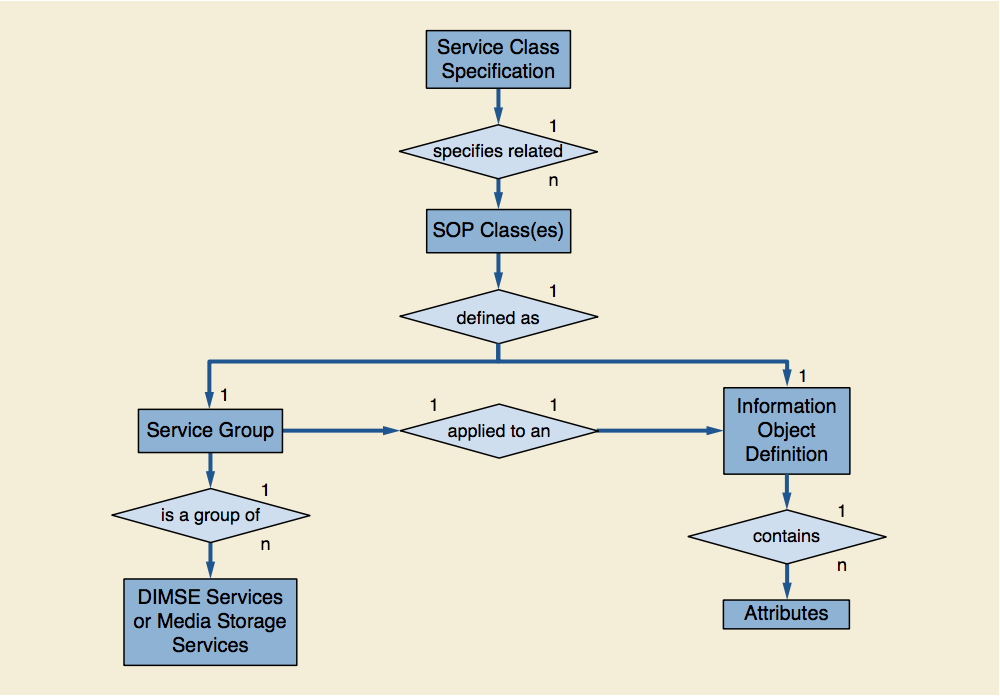
\includegraphics[width = 0.8\hsize]{./figures/DICOMInformationalModel}
\caption{DICOM Information Model Structure Representation}
\end{figure}


\begin{itemize}

\item The \textbf{DIMSE Service Group} specifies operations and notifications that are allowed on an Information Object Definition. \textbf{DIMSE} stands for DICOM Message Service Element and \textbf{Service Object Pair Classes} are used for message transfering between Information Object Definition.



\item \textbf{Information Object Definition} (IOD) are abstract objects which are intented to represent \textbf{instances of the real world model}. \textbf{Information Object Definition} can be made of one or more \textbf{Information Entities (IE)} - we talk about normalized vs composite IOD's. Each \textbf{Information Entities (IE)} and is made of \textit{attributes} describing a single piece of information. Information Entities are related to \textbf{real world object} for example a patient, and his attributes could be the patient name or date of birth. Attributes that have a link are grouped into \textbf{Information Object Module (IOM)}, which are defined in a way that they can be used in different IOD's. 

\end{itemize}


\clearpage

Figure 3 shows the representation of a Image (composite) IOD. Also, notice that all \textbf{DICOM Object} must at least contains the SOP common module and the four main \textbf{Information Entities}: Patient, Study, Serie and Image.


\newline \vspace{5mm}

\begin{figure}[ht]
\centering
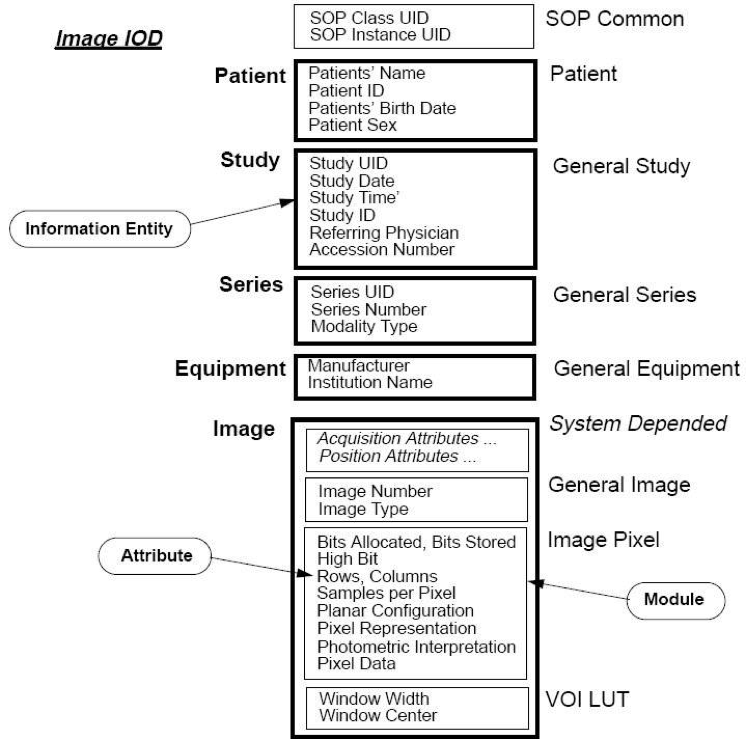
\includegraphics[width = 0.75\hsize]{./figures/ImageIOD}
\caption{Image IOD structure}
\end{figure}

\newline \vspace{5mm}

To more extend it is clear on the figure that each Information Entities has an attribute called UID, this stands for \textbf{Unique Identifier}. DICOM uses those identifiers to uniquely defines a wide variety of items to guaranty global uniqueness, mainly among different countries, sites, equipment.
